\section{Auftriebskraft}

\subsection{Grundlage der Auftriebskraft}
	Obwohl im Folgenden immer von der Auftriebskraft die Rede ist,
	wird in der Anwendung des Flügels immer nur den Querschnitt davon betrachtet,
	wie in Abbildung~\ref{joukowski:auftriebskraft:fig:kontourintegral-fluegel} zu sehen ist.
	Somit wird nicht die Kraft selbst,
	sondern die Kraft pro Flügellänge berechnet.
	Diese wird mit
	\[
		F'
		=
		\frac{\partial F}{\partial l}
	\]
	notiert.
	Um die resultierende Kraft pro Flügellänge zu erhalten,	
	müssen alle kleinen Kraftanteile $dF'$ um das geschlossene Profil des Flügels,
	welche wir mit $\gamma$ bezeichnen,
	aufsummiert werden, womit
	\begin{equation}
		F'
		=
		\displaystyle\oint_{\gamma}
		dF'
		\label{joukowski:auftriebskraft:Integral-aus-dF}
	\end{equation}
	entsteht.
	Aus der Bedingung, dass die Strömung reibungsfrei ist,
	wirken nur die Kraftanteile,
	welche normal zur Oberfläche des Flügels sind.
	Wirkt eine Kraft normal zu einer Oberfläche,
	so liegt einen Druck vor, welcher sich mit
	\[
		p
		=
		\frac{dF_\perp}{dA}
	\]
	berechnen lässt.
	Somit können wir den kleinen Kraftanteil $dF'$ durch den Druck $p(z)$ an diesem Punkt ausdrücken
	und es entsteht
	\[
		dF'
		=
		i \cdot p(z) dz,
	\]
	wobei jetzt Gleichung~\eqref{joukowski:auftriebskraft:Integral-aus-dF} als
	\begin{equation}
		F'
		=
		i \cdot \displaystyle\oint_{\gamma}
		p(z)
		dz
		\label{joukowski:auftriebskraft:Integral-aus-p}
	\end{equation}
	geschrieben werden kann.
	Mithilfe der Multiplikation mit $i$ können wir ausdrucken,
	dass jeder Kraftanteil immer nur senkrecht zur Umfahrtrichtung $dz$ wirkt,
	wie in Abbildung~\ref{joukowski:auftriebskraft:fig:kontourintegral-fluegel} dargestellt wird.
	
	\begin{figure}
	\centering
	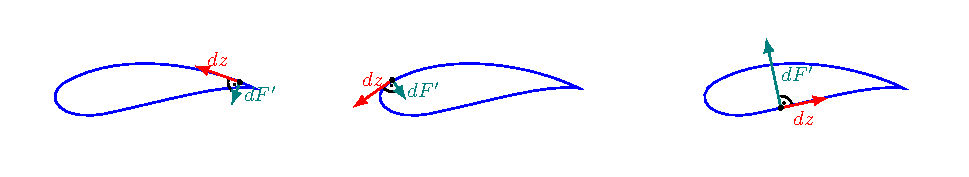
\includegraphics[width=\textwidth]{papers/joukowski/images/03_auftriebskraft/kontourintegral_fluegel.pdf}
	\caption{
		Die resultierende Kraft $F'$ ergibt sich durch das Aufsummieren aller kleiner Kraftanteilen $dF'$
		entlang der gesamten Kontur des Tragflügels.
		\label{joukowski:auftriebskraft:fig:kontourintegral-fluegel}}
\end{figure}


\subsection{Aus Anströmungsgeschwindigkeit wird Auftrieb}
	Bei der Betrachtung eines Objektes in einem beliebigen Medium kann eine Auftriebskraft festgestellt werden.
	Hierbei muss die Unterscheidung zwischen statischen und dynamischen Auftrieb gemacht werden.
	Der statische Auftrieb entsteht durch den Druckgradienten. 
	Dies ist auf den Druckunterschied zurückzuführen,
	wobei Strömungen zum dynamischen Auftrieb führen.
	
	Ein Beispiel für den statischen Druck ist ein Eiswürfel im Wasserglas. Der Druckgradient beschreibt die Druckveränderung zwischen zwei Punkten,
	daher kann relativ einfach über das verdrängte Volumen gerechnet werden.
		
	Bei einem Flugzeug ist dies wesentlich komplizierter.
	Hierbei handelt sich um dynamischen Auftrieb. Für die Strömung gilt Energieerhaltung.
	Der Druck, an einem beliebigen Punkt im Raum, kann somit mit der Bernoulli Gleichung
	
	\begin{equation}
		\label{joukowski:Auftriebskarft:Bernoulli}
		p(z) + \frac{\rho}{2} \cdot |v(z)|^2 + \rho g h(z) 
		=
		p_{\infty} + \frac{\rho}{2} \cdot |v_{\infty}|^2 + \rho g h_{\infty}
	\end{equation}
	beschrieben werden.
	Dabei werden immer zwei Punkte gewählt, in diesem Fall der Punkt $z$ und ein Punkt, in der Theorie unendlich, weit weg vom Flügelprofil. Wir können den Punkt in der Unendlichkeit auf der gleichen Höhe $h(z)$ wählen, somit verschwindet der statische Höhendruck. Aufgelöst nach dem Druck am Punkt $z$ ergibt sich die Form
	\[
		p(z)
		= 
		-\frac{\rho}{2} \cdot |v(z)|^2 + C,
	\]
	wobei der konstante Teil $C$ aus dem Referenzwert im Unendlichen besteht.
	Um nun die Auftriebskraft zu erhalten,
	kann die Formel für $p(z)$ in Gleichung~\eqref{joukowski:auftriebskraft:Integral-aus-p} eingesetzt werden,
	damit
	\begin{align}
		&F'
		=
		F_x' + i F_y'
		=
		- i \frac{\rho}{2} \cdot
		\displaystyle\oint_{\gamma}
		|v(z)|^2 + C \, dz 
		\notag
		\\
		\intertext{	entsteht.
					Der konstante Teil $C$ kürzt sich durch die Integration um die geschlossene Kontour $\gamma$ heraus.
					Übrig bleibt nur noch der Ausdruck}
		\label{joukowski:Auftriebskarft:Auftrieb1}
		&F'
		=
		F_x' + i F_y'
		=
		- i \frac{\rho}{2} \cdot
		\displaystyle\oint_{\gamma}
		|v(z)|^2 \, dz.
	\end{align}

